\documentclass[12pt]{beamer}
\usepackage[T1]{fontenc}
\usepackage[utf8]{inputenc}
\usepackage[polish]{babel}
\usepackage{multicol}
\usepackage{listings}
\usepackage{tabularx}

\definecolor{keywords}{RGB}{255,0,90}
\definecolor{comments}{RGB}{81,81,81}
\definecolor{offwhite}{RGB}{249,242,215}
\definecolor{foreground}{RGB}{255,255,255}
\definecolor{background}{RGB}{24,24,24}
\definecolor{title}{RGB}{107,174,214}
\definecolor{gray}{RGB}{155,155,155}
\definecolor{subtitle}{RGB}{102,255,204}
\definecolor{hilight}{RGB}{102,255,204}
\definecolor{vhilight}{RGB}{255,111,207}
\definecolor{lolight}{RGB}{155,155,155}
\setbeamercolor{titlelike}{fg=title}
\setbeamercolor{subtitle}{fg=subtitle}
\setbeamercolor{institute}{fg=gray}
\setbeamercolor{normal text}{fg=foreground,bg=background}
\setbeamercolor{item}{fg=foreground}
\setbeamercolor{subitem}{fg=gray}
\setbeamercolor{itemize/enumerate subbody}{fg=gray}
\setbeamertemplate{itemize subitem}{{\textendash}}
\setbeamerfont{itemize/enumerate subbody}{size=\footnotesize}
\setbeamerfont{itemize/enumerate subitem}{size=\footnotesize}

\title{\Huge{SFML}}
\subtitle{Biblioteka programistyczna}
\author{Patryk Sroczyński}
\institute{\large\textbf{Politechnika Śląska} \\
    Gliwice}
\date{}

\setbeamercovered{transparent=15}


\begin{document}
%\metroset{block=fill}



    \begin{frame}

        \titlepage

    \end{frame}



    \begin{frame}[t]{Czym jest SFML?}\vspace{20pt}

        \begin{center}
            
\includegraphics[scale=0.5]{textures/logo.png} \\[20pt]
        \end{center}
        

        \textbf{SFML} to akronim \textbf{Simple and Fast Multimedia Library} \\[20pt]

        Jest to wieloplatformowa biblioteka programistyczna ułatwiająca tworzenie gier
        oraz programów multimedialnych. \\[20pt]

        Autorem jest Laurent Gomila

    \end{frame}


    \begin{frame}[t]{Główne właściwości}\vspace{2pt}

        \begin{columns}
            
            \column{0.3\textwidth}
            
\includegraphics[scale=0.3]{textures/multimedia.png} \\[20pt]
            \begin{center}
                \textbf{Multi-media} \\
                Zawiera 5 modułów: system, window, graphics, audio i network
            \end{center}
            

            \column{0.3\textwidth}
            
\includegraphics[scale=0.3]{textures/multiplatform.png} \\[20pt]
            \begin{center}
                \textbf{Multi-platform} \\
                Można uruchomić oraz skompilować na Windowsie, Linuxie, macOS
            \end{center}

            \column{0.3\textwidth} \\[28pt]
            
\includegraphics[scale=0.3]{textures/multilanguage.png} \\[20pt]
            \begin{center}
                \textbf{Multi-language} \\
                Głównym językiem jest C++, ale można również zbindować np.: Java, Ruby, Python
            \end{center}

        \end{columns}

    \end{frame}



    \begin{frame}[t]{Moduły}\vspace{40pt}

        \begin{enumerate}
            \item \textit{System} – obsługuje czas i wątki
            \item \textit{Window} – obsługuje okna i interakcję z użytkownikiem
            \item \textit{Graphics} – umożliwia renderowanie grafiki
            \item \textit{Audio} – dostarcza interfejsu do odtwarzania muzyki i dźwięków
            \item \textit{Network} – odpowiedzialny za komunikację sieciową
        \end{enumerate}

    \end{frame}



    \begin{frame}[t]{Wybrane metody i właściwości klasy sf::RenderWindow}\vspace{4pt}

        \only<1>{
            Klasa sf::RenderWindow jest najważniejsza, ponieważ dzięki niej możemy
            stworzyć okno, a następnie wyświetlać zawartość \\[10pt]
            \begin{center}
                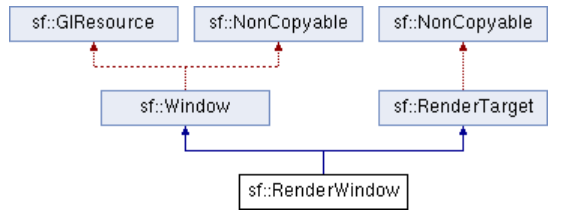
\includegraphics[scale=0.6]{textures/renderWindow.png}
            \end{center}
        }

        \only<2>{
            \begin{enumerate}
                \item konstruktor: sf::RenderWindow::RenderWindow( VideoMode, const String&, Uint32, const ContextSettings& ) 
                \item void clear(const Color &color=Color(0,0,0,255)) 
                \item void draw(const Drawable &drawable, const RenderStates &states=RenderStates::Default)
                \item void display()
                \item void setVerticalSyncEnabled(bool enabled)
                \item void setFramerateLimit(unsigned int limit)

            \end{enumerate}
        }

    \end{frame}



    \begin{frame}[fragile]
        \frametitle{Program tworzący puste okno}
        \lstset{language=C++,
                        basicstyle=\small\ttfamily,
                        keywordstyle=\color{blue}\ttfamily,
                        stringstyle=\color{red}\ttfamily,
                        commentstyle=\color{green}\ttfamily,
                        morecomment=[l][\color{magenta}]{\#},
                        numbers=left,
                        framexrightmargin=0em,
                        framexleftmargin=0em,
                        framerule=0pt
        }
        \begin{lstlisting}         
#include <SFML/Graphics.hpp>
 
int main() {
    sf::RenderWindow window(sf::VideoMode(800, 
    600), "Tytul");

    while (window.isOpen()) {
    sf::Event event;
        while (window.pollEvent(event)) {
            if (event.type == sf::Event::Closed)
                window.close();
        }       
        window.clear();       
        window.display();
    }
}

        \end{lstlisting}
    \end{frame}
    


    \begin{frame}[t]{Tworzenie prostych kształtów}

        \begin{table}
            \centering
            \def\arraystretch{2}
            \newlength\mylength
            \setlength\mylength{\dimexpr.5\columnwidth-20\tabcolsep-0.5\arrayrulewidth\relax}
            \begin{tabularx}{\columnwidth}{p{\mylength}||X|X|X}
                \hline
                Kształt & Wygląd & Kod & Rysowanie \\\hline

                \bigcirc & 
\includegraphics[scale=0.3]{textures/circle.png}
                & \scriptsize{sf::CircleShape circle(50.f);} 
                & \scriptsize{window.draw(circle);} \\\hline

                \Box & 
\includegraphics[scale=0.3]{textures/rect.png}
                 & \scriptsize{sf::RectangleShape rect(sf::Vector2f(50.f, 50.f));} 
                 & \scriptsize{window.draw(rect);} \\\hline

                \bigtriangleup & 
\includegraphics[scale=0.3]{textures/triangle.png} 
                & \scriptsize{sf::CircleShape triangle(80, 3);} 
                & \scriptsize{window.draw(triangle);} \\\hline

            \end{tabularx}
        \end{table}

    \end{frame}



    \begin{frame}

        \flushleft
        \huge{Dziękuję za uwagę!}

        \vspace{90pt}

        \large{Bibliografia:} \\

        \textcolor{green}{
            \url{https://www.sfml-dev.org/} \\
            \url{https://en.wikipedia.org/wiki/Simple_and_Fast_Multimedia_Library} \\
        }
        

    \end{frame}



\end{document}